\documentclass[12pt,reqno, twoside]{amsbook}
%%%%%%%%%%%%%%%%%%%%%%%%%%%%%%%%%%%%%%%%%%%%%%%%%%%%%%%%%%%%%%%%%%%%%%%%%%%%%%%%%%%%%%%%%%%%%%%%%%%%%%%%%%%%%%%%%%%%%%%%%%%%%%%%%%%%%%%%%%%%%%%%%%%%%%%%%%%%%%%%%%%%%%%%%%%%%%%%%%%%%%%%%%%%%%%%%%%%%%%%%%%%%%%%%%%%%%%%%%%%%%%%%%%%%%%%%%%%%%%%%%%%%%%%%%%%
\usepackage{eurosym}
\usepackage{amsmath}
\usepackage{amssymb}
\usepackage{amsfonts}
\usepackage[onehalfspacing]{setspace}
\usepackage{chngcntr}
\usepackage{graphicx}
\usepackage[a4paper, margin=2.5cm]{geometry}
\usepackage[english]{babel}
\usepackage{fancyhdr}
\usepackage{titlesec}
\usepackage{enumitem}
\usepackage{etoolbox}
\usepackage{comment}
\usepackage{caption}
\usepackage{enumitem}
% you may need to uncomment the command below if you use eps format for figures
%\usepackage{epstopdf}

\makeatletter
\def
\section{\@startsection{section}{1}%
  \z@{.5\linespacing\@plus.7\linespacing}{.25\linespacing}%
{\normalfont\bfseries\flushleft}}
\def
\subsection{\@startsection{subsection}{2}%
  \z@{.5\linespacing\@plus.7\linespacing}{.25\linespacing}%
{\normalfont\bfseries\flushleft}}

\makeatother
\setcounter{MaxMatrixCols}{10}

\providecommand{\U}[1]{\protect\rule{.1in}{.1in}}
\theoremstyle{plain}
\newtheorem{acknowledgement}{Acknowledgement}
\newtheorem{algorithm}{Algorithm}[chapter]
\newtheorem{axiom}{Axiom}[chapter]
\newtheorem{case}{Case}[chapter]
\newtheorem{claim}{Claim}[chapter]
\newtheorem{conclusion}{Conclusion}[chapter]
\newtheorem{condition}{Condition}[chapter]
\newtheorem{conjecture}{Conjecture}[chapter]
\newtheorem{corollary}{Corollary}[chapter]
\newtheorem{criterion}{Criterion}[chapter]
\newtheorem{definition}{Definition}[chapter]
\newtheorem{example}{Example}[chapter]
\newtheorem{exercise}{Exercise}[chapter]
\newtheorem{lemma}{Lemma}[chapter]
\newtheorem{notation}{Notation}[chapter]
\newtheorem{problem}{Problem}[chapter]
\newtheorem{proposition}{Proposition}[chapter]
\newtheorem{remark}{Remark}[chapter]
\newtheorem{solution}{Solution}[chapter]
\newtheorem{summary}{Summary}[chapter]
\newtheorem{theorem}{Theorem}[chapter]
\numberwithin{equation}{chapter}

% Please write the references according to your school

\newenvironment{dedication}
{%\clearpage           % we want a new page
  \thispagestyle{empty}% no header and footer
  \vspace*{\stretch{1}}% some space at the top
  \itshape             % the text is in italics
  \raggedleft          % flush to the right margin
}
{\par % end the paragraph
  \vspace{\stretch{3}} % space at bottom is three times that at the top
  %\clearpage           % finish off the page
}
\numberwithin{section}{chapter}
\fancyhead{}
\fancyfoot{}
\pagestyle{fancy}
\fancyfoot[LE,RO]{\thepage}

\makeatletter
\def\ps@plain{\ps@empty
  \def\@evenfoot{%
    \normalfont\scriptsize
    \rlap{\thepage}\hfil
  }%
  \def\@oddfoot{%
    \normalfont\scriptsize \hfil
  \llap{\thepage}}%
}
\makeatother
\renewcommand{\headrulewidth}{0pt}
\renewcommand{\footrulewidth}{0pt}

\begin{document}
\frontmatter
\addtocontents{toc}{\setcounter{tocdepth}{2}}
\thispagestyle{empty}

\begin{dedication}%

  \begin{flushright}
    \textit{Write here your dedication!}
  \end{flushright}%
\end{dedication}

\setcounter{page}{1}
\pagenumbering{roman} %
\chapter*{Cover}

\chapter*{Acknowledgment}

Write here the acknowledgments and grants, if any

\chapter*{Resumo}

Write here your abstract in Portuguese

\chapter*{Abstract}

Write here your abstract in English

\tableofcontents

\mainmatter
\setcounter{page}{1} \pagenumbering{arabic}

\chapter{Introduction}
\noindent The digital transformation of educational institutions has created new opportunities for integrating analytics and gamification in order to improve learning outcomes.
The Learning Scorecard (LS) platform embodies this approach, merging business intelligence with educational strategies to monitor and enhance student engagement and performance.

This thesis presents the development of the Learning Scorecard v2.5: a
prototype plugin that integrates some of the major features of the previous LS
iterations with the Moodle Learning Management System Service API.\@
\section{Motivation}
\section{Statement of the Problem}
\section{Aims and Objectives}
\section{Methodological Approach}
\section{Structure of the Thesis}

\chapter{Literature Review}
\section{Learning Management Systems}
\noindent Learning Management Systems (LMS) represent sophisticated software applications engineered to administer, track, report, automate, and deliver educational courses, training programs, and comprehensive learning materials. Following their initial emergence in the late 1990s, these platforms have achieved near-universal adoption across higher education institutions globally. Recently, the unprecedented expansion of LMS usage has been significantly accelerated by the institutional shift toward remote learning by the COVID-19 pandemic.

There are a plethora of LMS available for educational institutions, with
ommercial and open-source platforms representing the two primary categories of
LMS offerings~\cite{mohd_kasim_choosing_2016}. Commercial LMS are either
available in the market for a price or, although very rarely, proprietary and
developped by the institution. In contrast, the open source alternative is
available at no cost to the institution, although technical expertise is
required aswell as regular functional assessments. Open-source systems provide
publicly accessible source code that institutions can modify and improve to
meet their specific requirements and needs \cite{cavus_comparison_2014}.

Moodle (Modular Object-Oriented Dynamic Learning Environment) stands as one of
the most widely adopted open-source learning management systems globally.
According to a recent systematic review on tendencies in the use of LMS, Moodle
is the most popular and preferred open-source
LMS~\cite{altinpulluk_systematic_2021}. The platform's extensive reach is
evidenced by its current deployment across 238 countries, serving approximately
468 million users worldwide~\cite{moodle_stats_2025}.

\begin{figure}[h]
  \centering
  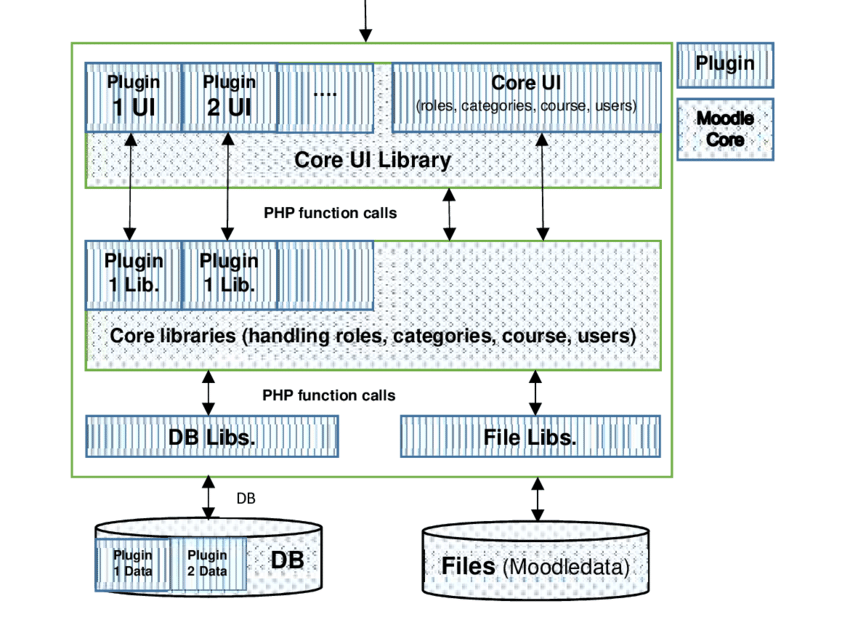
\includegraphics[width=0.8\textwidth]{images/Moodle-three-tier-architecture.png}
  \caption{Moodle three tier architecture. Source: Dolawattha et al.~\cite{dolawattha_impact_2019}.}
  \label{fig:moodle_arch}
\end{figure}

From a technical perspective, Moodle is built on a layered architecture that
ensures flexibility and scalability. The presentation layer handles the user
interface and allows users to interact both on desktop and mobile devices. The
application layer accommodates core functionalities and acts as an intermediary
between the presentation and data layer, supporting the installation of plugins
and modules to customize features. The data layer includes the database
management system, typically SQL-based, which stores and manages all the data.
This modular design allows institutions to customize the functionality and
appearance through a extensive plugin ecosystem.

Moodle offers many plugins that allow for functionality expansion. There are
multiple types of plugins from local plugins, block plugins all the way to
antivirus plugins. Each with its own purpose and place in the moodle folder
structure.

\section{Gamification and Motivation in Education}
\subsection{Theoretical Perspectives on Gamification}
\subsection{Gamification and Student Engagement}

\chapter{The Learning Scorecard: Concept and Evolution}
\section{Genesis and Conceptualization of the Learning Scorecard}
\noindent The Learning Scorecard emerged from a fundamental pedagogical challenge identified within higher educational institutions: the lack of understanding by faculty members regarding the difficulties experienced by students in relations to the content taught in curricular units aswell as the students disinterest and lack motivation. Initially, this platform was conceptualized as a comprehensive academic performance management system designed to support both students and faculty through data-driven insights that assist educators in continuously monitoring the curricular units they teach while enabling students to visualize their performance in each course in which they are enrolled. Their main mission was to offer higher education students an analytic environment that allows progress monitorization in a curricular unit, contributing for a better learning experience.

The platform was originally conceptualized with three distinct user
perspectives: student view, teacher view, and administrative view. The student
view provides essential visualizations that enable students to understand their
learning trajectory in a specific curricular unit while offering tools that
provide important data for continuous monitoring by faculty. The teacher view
provides management, evaluations and visualization tools for educators
regarding each curricular unit they teach, offering various visualizations to
track each students progress through all phases of the curricular unit along
with assessment tools.

\section{Evolution Through Iterative Development}
\subsection{Historical Overview of Versions}
\noindent The Learning Scorecard development followed a systematic timeline beginning in the 2015/16 academic year by a group of Computer Science masters students attending the Informatic Systems of Decision Support II curricular unit. The platform evolved through \textbf{X} major versions, each incorporating lessons from previous iterations and expanding functionality based on user feedback.

\textbf{Learning Scorecard Version 1 (2016)}

\textbf{Learning Scorecard Version 2 (2017)}

\textbf{Learning Scorecard Version 3 (2018)}

\subsection{Lessons Learned from Prior Iterations}
\section{Learning Scorecard Conceptual Framework}

The Learning Scorecard (LS) conceptual framework encompasses a comprehensive
set of interconnected concepts designed to support gamified learning
experiences in higher education. These concepts can be organized into four
primary domains: Academic Structure, Gamification Mechanics, Social Learning,
and Performance Recognition.

\subsection{Academic Structure and Organization}

The academic foundation of the Learning Scorecard is built upon traditional
higher education organizational structures, adapted to support digital learning
environments.

\textbf{Courses and Curricular Units.} The system recognizes a two-tier academic structure where \textit{Courses} represent overarching academic programs (e.g., "Computer Science") that encompass multiple \textit{Curricular Units}. Each Curricular Unit corresponds to an individual subject with specific learning objectives, content, and assessments that students must complete as part of their academic progression. This hierarchical organization maintains consistency with traditional academic frameworks while enabling digital tracking and gamification.

\textbf{Students and Faculty.} The system accommodates two primary user roles: \textit{Students}, who are enrolled in one or more Curricular Units and participate in gamified learning activities, and \textit{Teachers} or Faculty members, who are responsible for creating and managing curricular content, designing learning activities, and monitoring student progress within their assigned Curricular Units.

\textbf{Syllabus Contents, Calendar and Timeline.} \textit{Syllabus Contents} encompass all learning materials, resources, and educational content within a Curricular Unit. The organizational framework includes both \textit{Calendar} and \textit{Timeline} concepts that serve as complementary planning systems, enabling students and faculty to organize learning activities and maintain temporal awareness of curricular progression.

\subsection{Gamification Mechanics}

The core gamification elements provide the foundation for student engagement
and progress tracking through game-like mechanics adapted to educational
contexts.

\textbf{Experience Points and Ranks.} \textit{Experience Points} (XP) serve as the fundamental currency of progress within the platform, earned through completion of various educational activities. The \textit{Rank} system establishes hierarchical progression levels based on accumulated XP, including ranks such as Newbie (entry level at 0 XP), Rookie, Skilled Expert, Master, and Legendary. Faculty members can configure rank thresholds dynamically, with each rank unlocking new privileges and recognition within the platform.

\textbf{Quests.} \textit{Quests} represent the core educational activities that students complete to earn XP and demonstrate learning. The system categorizes quests into five distinct types: Class Attendance, Practical Assignment, Quiz, Exercise, and Event. Each quest can be designated as mandatory (milestone quests) or optional, providing flexibility in curriculum design while maintaining educational objectives.

\textbf{Last Chances.} The \textit{Last Chance} mechanism provides opportunities for recovery and continued engagement when students fall behind or make mistakes, preventing permanent failure states that could lead to disengagement and ensuring continued participation throughout the academic term.

\subsection{Social Learning Framework}

The social components of the Learning Scorecard foster collaboration and
healthy competition among students through structured group dynamics.

\textbf{Alliances.} \textit{Alliances} function as large-scale organizational units that typically correspond to academic classes or programs (e.g., LEI or ETI). These structures facilitate competition and comparison at the class level while maintaining educational coherence, enabling students to compare their progress through dedicated leaderboards and participate in alliance-specific activities.

\textbf{Guilds.} \textit{Guilds} represent smaller collaborative units within alliances, typically corresponding to project teams or study groups. The guild system promotes cooperative learning by encouraging mutual assistance among members, with guild-specific achievements, badges, and leaderboards fostering team spirit while maintaining individual accountability within the collaborative framework.

\subsection{Recognition and Achievement System}

The recognition framework provides multiple pathways for acknowledging student
accomplishments and maintaining motivation through visible achievements.

\textbf{Badges.} The \textit{Badge} system provides targeted recognition for specific accomplishments and behaviors, featuring 39 different badges organized into four categories: individual achievements, guild-based accomplishments, forum participation, and final questionnaire completion. Each category includes multiple tiers (bronze, silver, gold, and platinum) corresponding to increasing levels of difficulty and commitment.

\textbf{Trophies.} \textit{Trophies} represent the highest level of achievement, awarded to top performers in various leaderboard categories including overall rankings (Best Score Player), guild performance (Best Guild), and combined metrics (Best Triathlon Player). Each trophy provides substantial XP rewards (typically 1000 XP) and serves as a highly visible symbol of excellence.

\textbf{Avatars.} The \textit{Avatar} system enables profile customization while serving as a visual indicator of progression. Students unlock new avatar options as they advance through rank levels, with both male and female options available at each tier, allowing for personal expression while maintaining the connection between visual representation and academic achievement.

\textbf{Leaderboards.} Multiple \textit{Leaderboard} systems enable various forms of competition and comparison through five distinct categories: overall individual rankings, guild-based comparisons, exercise-specific performance, quiz results, and combined metrics. Each leaderboard displays position, username, rank, avatar, and XP totals, creating transparency in academic performance while fostering healthy competition among participants.

\begin{comment}
\subsection{Monitoring and Analytics}

\subsubsection{Student Dashboard}
\paragraph\ The student dashboard serves as the central interface for progress monitoring and decision-making.
Students can view their advancement across different quest types, track XP accumulation, monitor rank progression, and analyze their performance relative to peers.
The dashboard integrates all gamification elements into a cohesive user experience.

\subsubsection{History Tracking}
\paragraph\ The platform maintains comprehensive records of all student activities and achievements.
The history system allows students to review their XP gains from each quest, track their progression over time, and understand the relationship between their efforts and outcomes.

\subsection{Faculty Management}

\subsubsection{Quest Configuration}
\paragraph\ Faculty members can create and manage quests through both individual interfaces and bulk Excel imports.
The system allows for dynamic quest addition throughout the term, enabling responsive curriculum adjustment based on student needs and learning objectives.

\subsubsection{Rank and XP Configuration}
\paragraph\ Instructors have comprehensive control over rank thresholds and XP distribution.
This flexibility enables adaptation to different course structures, student populations, and learning objectives while maintaining game balance and engagement.

\subsection{Assessment Integration}

\subsubsection{Continuous Assessment Connection}
\paragraph\ The gamification system integrates directly with academic assessment, allowing XP and rank progression to contribute to final course grades.
This connection ensures that game mechanics support rather than distract from educational objectives.

\subsubsection{Difficulty and Challenge Scaling}
\paragraph\ The platform incorporates mechanisms for adjusting challenge levels and providing appropriate difficulty progression.
This ensures that all students can find appropriate challenges while maintaining engagement across diverse skill levels and learning paces.
\end{comment}

\chapter{System Architecture and Design}
\section{Requirements}
\noindent An imperative aspect in any application conceptualization is a thorough requirement analysis. These requirements can be functional (FR) or non functional (NFR) and shape the architectural decisions that are made during its development as well as assessing whether a system will succeed.

\textbf{Functional Requirements (FR)}

It's important to define what an engineer should strive for when determining
functional requirements as it will ultimately be what defines an application,
molds its functionality and consequently decides it's architecture. Functional
requirements are the essential characteristics that the system should deliver
that the end-user specifically demands.~\cite{saroja_functional_2023} A simpler
way to perceive it is that they define what the system should perform. It's
important with any version increment of the LS to maintain fidelity to the
previous requirements and adjust them when appropriate.
Costa~\cite{costa_thesis_2017} identified base functional requirements which I
will evaluate and integrate into my system architecture, but also define some
myself. From Costa's functional requirements:
\begin{enumerate}
  \item Users must have a profile and authentication credentials
  \item The LS platform must be integrated with the e-learning system (access to quiz
        results, forum participation, material download, etc)
  \item There must exist two types of accounts: student and teacher/faculty
  \item The LS platform must have a dashboard for individual student performance
        monitorization (students view)
  \item The LS platform must have a dashboard for class performance monitorization
        (teacher view)
  \item The LS platform must have a course chronogram with deadlines and study
        guidelines, personalized by the teacher/faculty
  \item The LS platform must include gamification elements (score, ranks, quests,
        leaderboards)
\end{enumerate}
At first glance, we can satisfy the requirements 1,2 and 3 just with the new LS version integrated as a moodle plugin. The first requirement specifies the necessity of a profile and authentication credentials. Every student receives a moodle account aswell as authentication credentials at the start of each new course year. The second requirement is also already satisfied as the LS 2.5 version will be a plugin of moodle, therefore it will be integrated with the e-learning system by itself. Lastly, the third requirement we can already satisfy is also a base moodle functionality. All accounts are user accounts although their role (student, teacher, etc) limits what they can access.

\textbf{Non-Functional Requirements (FR)}

Another important aspect of the requirement analysis is to define the
non-functional requirements. These, differently from their functional
counterpart must define how the system should perform, rather than what. While
not directly visible as features they are vital in shaping the user experience
and ensuring the system's long-term success. A few examples of these
requirements could be performance, security, reliability, etc.
Costa~\cite{costa_thesis_2017} also layed out base non-functional requirements
which I will also evaluate, adapt and integrate into my system architecture, in
addition to some identified by myself. From Costa's non-functional
requirements:
\begin{enumerate}
  \item Portability for the different web browsers, including mobile devices
  \item Intuitive and user-friendly interface (least possible manual input by students)
  \item The user identification data must be private (ethical requirement), the
        teacher/faculty must only have access to the class agregated data, even for at
        risk students.
\end{enumerate}
This last non-functional requirement, as Costa correctly identified is a missed opportunity as the faculty will have no way of knowing which student is at risk
and ultimately take advantage of such introspective metrics on student performance. As the system is integrated into moodles learning environment and all this information is already available to the faculty I believe this NFR should be altered into a more transparent requirement.
\section{Overview of LS Architecture}
\section{Moodle Development Environment}
\noindent The first challenge faced when beginning the development of any new system is to configure the development environment. This task usually begins with setting up a source code management (SCM) system, like Git~\cite{git_scm} and configuring your IDE with the correct formatting, intellisense and file structure.
The moodle plugin development has brought up some additional effort as a moodle instance is required.

It was imperative to configure a stable, consistent and mature moodle instance,
in order to develop the plugin against a production-like environment, mimicking
the ISCTE moodle instance as much as possible. After some investigation I
determined that the ISCTE moodle 2024/2025 version was 4.4.1.

Firstly I used the application XAMPP~\cite{apache_friends_xampp} in order to
have a PHP environment, an apache server and a MariaDB~\cite{mariadb_database}
server in which to execute and manage the moodle instance as a standalone
application. The behavior was abnormal and unpredictable. After every restart
of the server the files weren't persisted and it didn't allow for a stable,
consistent and reproducible development environment.

On the second attempt, with Docker~\cite{docker_containers} and container
orchestration and a registered bitnami image~\cite{bitnami_cloud} (a
production-ready open source software deliverer) the results were much more
favorable and allowed me to restart and stop the container with the moodle and
the database instances persisting. Unfortunately, when the plugin was added to
the image files the moodle configurer assumed the moodle files were corrupted
and attempted a fresh installation. Again, it wasn't up-to the standards of a
production-like environment.

Finally, the solution that provided the best results and closer production-like
environment was using Docker with an apache server image where I manually
configured the moodle instance and a MariaDB database image as it proved to be
reliable, stable and consistent. During my research I found that the moodle
configurer attemping the fresh installation was a bitnami image bug that was
unsolved by the developers and not a moodle problem.

Now, with an environment I could rely on and a safer, more consistent and
easier to debug moodle instance I was finally able to begin integrating and
developing a moodle plugin.

\section{Plugin Integration with Moodle}
\noindent There are multiple types of moodle plugins and depending on their purpose we should select the most adequate. According to the specification of the Learning Scorecard we would need to evaluate what plugin type is better suited.

The functionality of user metrics appearing on a student or a teacher dashboard
would be a perfect application for a Block Plugin. From the moodle
dev~\cite{moodle_plugin_api} API guide it is mentioned that the blocks are
small information-displays or tools that can be moved around pages. It would
then be available to integrate into each users dashboard and customize in a
widget like manner.

When it comes to the leaderboards and learning scorecard settings (xp, badge
and leaderboard) a local plugin would be the better choice as, according to the
moodle dev plugin specification they are generic plugins for local
customisations.

Depending on the type of plugin, their installation location will also vary.
For the block plugin the localtion will be inside a directory called
\textit{"/blocks"} and in turn, the local plugin should be inside the
\textit{"/local"} directory.

\subsection{Concept Mapping}
\centering
\begin{center}
  \captionof{table}{Learning Scorecard vs Moodle Concept Mapping}
  \begin{tabular}{ccc}
    Concept            & Moodle                               & Feasibility \\ \hline
    \multicolumn{3}{c}{\textit{Academic}}                                   \\
    Course             & Course Categories                    & T           \\
    Curricular Unit    & Course                               & T           \\
    Student            & Users \& Roles                       & T           \\
    Teacher / Faculty  & Users \& Roles                       & T           \\
    Syllabus Contents  & Course Modules \& Tags               & T           \\
    Calendar           & Calendar Events                      & P           \\
    Timeline           & Activity Completion \& Progress      & P           \\
    \multicolumn{3}{c}{\textit{Gamification}}                               \\
    Experience Points  & Grade Items \& Custom Fields         & P           \\
    Ranks              & Custom Implementation                & P           \\
    Quests             & Activities                           & T           \\
    Alliances          & Groups \& Cohorts                    & T           \\
    Guilds             & Groups                               & T           \\
    Badges             & Badges System                        & T           \\
    Trophies           & Badges System \& Custom Impl.        & P           \\
    Avatars            & User Profiles, Files \& Custom Impl. & P           \\
    Leaderboards       & Gradebook \& Custom Views            & P           \\
    Last Chance System & Conditional Activities               & P
  \end{tabular}
  \caption*{T - Total Mapping  P - Partial Mapping}
\end{center}

\section{Database Design and Data Flow}
\section{Security and Scalability Considerations}\

\chapter{MVP}
\section{System Components and Modular Design}
\subsection{Student Interface and Experience}
\subsection{Teacher Dashboard and Analytics}
\subsection{Administrator Functions and Control}

\chapter{Evaluation and Results}
\section{Demonstration of Key Features}
\section{Use Cases: Pilot Deployments and User Stories}
\section{Feedback and Empirical Results}
\section{Comparative Analysis with Previous Approaches}
\section{Discussion of Evaluation Metrics}

\chapter{Conclusions}
\section{Summary of Contributions}
\section{Limitations and Challenges}
\section{Future Directions for LS}

\renewcommand{\bibname}{References}

\def\bibindent{0.7cm}
\begin{thebibliography}{99\kern\bibindent}
  \makeatletter
  \let\old@biblabel\@biblabel
  \def\@biblabel#1{\old@biblabel{#1}\kern\bibindent}
  \let\old@bibitem\bibitem
  \def\bibitem#1{\old@bibitem{#1}\leavevmode\kern-\bibindent}
  \makeatother
  \makeatletter
  \renewcommand\@biblabel[1]{}
  \makeatother

  \bibitem{mohd_kasim_choosing_2016} N.N. Mohd Kasim and F. Khalid (2016), \textquotedblleft Choosing the Right Learning Management System (LMS) for the Higher Education Institution Context: A Systematic Review\textquotedblright, \textit{International Journal of Emerging Technologies in Learning (iJET)}, 11(6), 55.

  \bibitem{cavus_comparison_2014} N. Cavus and T. Zabadi (2014), \textquotedblleft A Comparison of Open Source Learning Management Systems\textquotedblright, \textit{Procedia - Social and Behavioral Sciences}, 143, 521--526.

  \bibitem{altinpulluk_systematic_2021} H. Altinpulluk and M. Kesim (2021), \textquotedblleft A Systematic Review of the Tendencies in the Use of Learning Management Systems\textquotedblright, \textit{Turkish Online Journal of Distance Education}, 22(3), 40--54.

  \bibitem{moodle_stats_2025} Moodle (2025), \textquotedblleft Moodle Statistics\textquotedblright, Available at: https://stats.moodle.org/ (Accessed: 6 August 2025).

  \bibitem{dolawattha_impact_2019} D.D.M. Dolawattha, H.K.S. Pramadasa, and P.M. Jayaweera (2019), \textquotedblleft The Impact Model: Teachers' Mobile Learning Adoption in Higher Education\textquotedblright, \textit{International Journal of Education and Development using Information and Communication Technology (IJEDICT)}, 15(4), 71--88.

  \bibitem{saroja_functional_2023} S. Saroja and S. Haseena (2023), \textquotedblleft Functional and Non-Functional Requirements in Agile Software Development\textquotedblright, in \textit{Agile Software Development}, John Wiley \& Sons, Ltd, pp. 71--86.

  \bibitem{costa_thesis_2017} D.S. Costa (2017), \textquotedblleft Learning Scorecard: Plataforma para a Monitorização da Experiência de Aprendizagem de Alunos no Ensino Superior Aplicando Técnicas de Business Intelligence e Gamificação\textquotedblright, Master's Thesis, ISCTE-IUL, Lisbon, Portugal.

  \bibitem{git_scm} Git Community (2024), \textquotedblleft Git: Distributed Version Control System\textquotedblright, Available at: https://git-scm.com/.

  \bibitem{apache_friends_xampp} Apache Friends (2024), \textquotedblleft XAMPP Apache + MariaDB + PHP + Perl\textquotedblright, Available at: https://www.apachefriends.org/.

  \bibitem{docker_containers} Docker Inc. (2024), \textquotedblleft Docker: Accelerated Container Application Development\textquotedblright, Available at: https://www.docker.com/.

  \bibitem{bitnami_cloud} Bitnami (2024), \textquotedblleft Bitnami: Packaged Applications for Any Platform\textquotedblright, Available at: https://bitnami.com/.

  \bibitem{mariadb_database} MariaDB Foundation (2024), \textquotedblleft MariaDB Server: The Open Source Relational Database\textquotedblright, Available at: https://mariadb.org/.

  \bibitem{moodle_plugin_api} Moodle Pty Ltd (2024), \textquotedblleft Plugin Types API Documentation\textquotedblright, Moodle Developer Resources, Available at: https://moodledev.io/docs/4.1/apis/plugintypes.
\end{thebibliography}

\end{document}
